%%%%%%%%%%%%%%%%%%%%%%%%%%%%%%%%%%%%%%%%
% Mercury Requirements
% 20 minute talk for Bioinformatics Analysis Pipelines Day
% Wellcome Trust Sanger Institute
% 24th July 2014
% Joshua C. Randall
% 
% This work is licensed under the Creative Commons Attribution-ShareAlike 4.0 
% International License. To view a copy of this license, visit 
% http://creativecommons.org/licenses/by-sa/4.0/.
%
% It should be attributed to Joshua C. Randall, Genome Research Limited.
%
% It includes some images which are used under license and which are 
% available separately under their own license terms (all are CC licenses).
% 
% Comments next to each image included in this document cite the source.
% 
%%%%%%%%%%%%%%%%%%%%%%%%%%%%%%%%%%%%%%%%
\documentclass[xcolor=x11names,compress]{beamer}

\usepackage{graphicx}
\DeclareGraphicsExtensions{.pdf,.png,.jpg}
\usepackage{xcolor}
\usepackage{overpic}

% Sanger colour palette
\definecolor{sangerdarkblue}{RGB}{0, 72, 105}
\definecolor{sangermidblue}{RGB}{138, 187, 238}
\definecolor{sangerlightblue1}{RGB}{159, 198, 238}
\definecolor{sangerlightblue2}{RGB}{184, 210, 239}
\definecolor{sangerlightblue3}{RGB}{203, 220, 230}
\definecolor{sangerlightteal}{RGB}{176, 227, 192}
\definecolor{sangerlimegreen}{RGB}{204, 242, 132}
\definecolor{sangerolivegreen}{RGB}{95, 128, 17}
\definecolor{sangerdarkteal}{RGB}{5, 122, 82}
\definecolor{sangermintgreen}{RGB}{221, 246, 164}
\definecolor{sangerdarkbrown}{RGB}{132, 109, 83}
\definecolor{sangerlightbrown}{RGB}{204, 179, 118}
\definecolor{sangerdarkmustard}{RGB}{132, 93, 0}
\definecolor{sangerredbrown}{RGB}{98, 23, 0}
\definecolor{sangerorange}{RGB}{255, 114, 0}
\definecolor{sangerred}{RGB}{195, 0, 29}
\definecolor{sangerdarkred}{RGB}{141, 0, 23}
\definecolor{sangerpurple}{RGB}{124, 0, 79}

% Beamer Layout 
\useoutertheme[subsection=false,shadow]{miniframes}
\useinnertheme{default}
\usefonttheme{serif}
\usepackage{palatino}

\setbeamerfont{title like}{shape=\scshape}
\setbeamerfont{frametitle}{shape=\scshape}

\setbeamercolor*{background canvas}{bg=black}

\setbeamercolor*{lower separation line head}{bg=sangerdarkblue} 
\setbeamercolor*{normal text}{fg=white, bg=black} 
\setbeamercolor*{alerted text}{fg=red} 
\setbeamercolor*{example text}{fg=white} 
\setbeamercolor*{structure}{fg=sangerlightblue2} 
 
\setbeamercolor*{palette tertiary}{fg=black,bg=black!10} 
\setbeamercolor*{palette quaternary}{fg=black,bg=black!10} 

\renewcommand{\(}{\begin{columns}}
\renewcommand{\)}{\end{columns}}
\newcommand{\<}[1]{\begin{column}{#1}}
\renewcommand{\>}{\end{column}}

% title page colours
\newcommand{\titlepagefgcolour}{white}
\setbeamercolor*{title}{fg=\titlepagefgcolour}
\setbeamercolor*{subtitle}{fg=\titlepagefgcolour}
\setbeamercolor*{author}{fg=\titlepagefgcolour}
\setbeamercolor*{institute}{fg=\titlepagefgcolour}
\setbeamercolor*{date}{fg=\titlepagefgcolour}

% backgroundblock environment for background images
% from: "beamer: How to place images behind text (z-order)"
% (http://tex.stackexchange.com/a/134311)
\makeatletter
\newbox\@backgroundblock
\newenvironment{backgroundblock}[2]{%
  \global\setbox\@backgroundblock=\vbox\bgroup%
    \unvbox\@backgroundblock%
    \vbox to0pt\bgroup\vskip#2\hbox to0pt\bgroup\hskip#1\relax%
}{\egroup\egroup\egroup}
\addtobeamertemplate{background}{\box\@backgroundblock}{}
\makeatother


\begin{document}


%%%%%%%%%%%%%%%%%%%%%%%%%%%%%%%%%%%%%%%%
% Introduction
%%%%%%%%%%%%%%%%%%%%%%%%%%%%%%%%%%%%%%%%
\section*{\scshape Introduction}
\begin{frame}
\title{Mercury Requirements}
\subtitle{Bioinformatics Analysis Pipelines Day}
\author{
	Joshua C. Randall \\
	{\it 
	Human Genetics Informatics \\
	Wellcome Trust Sanger Institute 
	}\\
}
\date{
	% HGI logo is covered under the license for this work
	\scalebox{0.5}{
\includegraphics{HGI-ltblue}} \\
	\vspace{0.5cm}
	24th July 2014
}
\titlepage
\end{frame}

% HGI logo in bottom left corner of remaining frames
\addtobeamertemplate{background}{\vbox to0pt{\vskip 8.9cm \hbox to0pt{\hskip 1mm \relax
	% HGI logo is covered under the license for this work
	
\includegraphics[height=0.6cm]{HGI-ltblue}
}}}

% pipework background image
\newcommand{\pipesbackground}{
	\begin{backgroundblock}{0cm}{0cm}
		\vbox to \paperheight{\vfil\hbox to \paperwidth{\hfil
		\begin{overpic}[height=0.85\paperheight]{images/Jano_De_Cesare_-_Pipelines_-_by-nc-nd-2_0_-_flickr}
		% Image source: https://www.flickr.com/photos/janodecesare/3020406104/
		\put(88,0.5){\textcolor{gray}{\fontsize{4}{6}\selectfont Photo: Jano De Cesare}}
		\end{overpic}
		\hfil\hskip 2mm}\vfil}
	\end{backgroundblock}
}

\begin{frame}{Introduction}
\pipesbackground
\tableofcontents
\end{frame}


%%%%%%%%%%%%%%%%%%%%%%%%%%%%%%%%%%%%%%%%
% Background
%%%%%%%%%%%%%%%%%%%%%%%%%%%%%%%%%%%%%%%%
\section{\scshape Background}


%%%%%%%%%%%%%%%%%%%%%%%%%%%%%%%%%%%%%%%%
\subsection{What is a pipeline?}
\begin{frame}{What is a pipeline?}
\pipesbackground
\begin{itemize}
\item Recipe for producing data products from input data
\item Series of steps to be run in order
\item Represents analysis ``Best practices''
\item Can be run on different datasets to yield comparable results
\item In other fields this is often called a ``workflow''
\end{itemize}
\end{frame}

%%%%%%%%%%%%%%%%%%%%%%%%%%%%%%%%%%%%%%%%
\subsection{Pipeline system interfaces}
\begin{frame}{Pipeline system interfaces}
\pipesbackground
\begin{itemize}
\item Push vs Pull
\item Imperative vs Declarative
\item Procedural/RO vs Functional/RT
\item Inherently distributed or not 
\end{itemize}
\end{frame}

%%%%%%%%%%%%%%%%%%%%%%%%%%%%%%%%%%%%%%%%
\subsection{Pipeline systems in use today}
\begin{frame}{Pipeline systems in use today}
\pipesbackground
\begin{itemize}
\item Shell scripts
\item Make
\item LSF
\item Runner.pm
\item Other ad-hoc LSF wrappers
\item VRPipe
\item GATK/Queue
\item eHive
\end{itemize}
\end{frame}


%%%%%%%%%%%%%%%%%%%%%%%%%%%%%%%%%%%%%%%%
% Requirements
%%%%%%%%%%%%%%%%%%%%%%%%%%%%%%%%%%%%%%%%
\section{\scshape Requirements}
\begin{frame}{Core Requirements \\
(PRIOS)}
\begin{backgroundblock}{0cm}{0cm}
		\vbox to \paperheight{\vfil\hbox to \paperwidth{\hskip 6cm 
		\begin{overpic}[height=0.85\paperheight]{images/Tom_Arthur_-_Shirt_and_Shoes_Required_-_by-nc-sa-2_0_-_flickr}
		% Image source: https://www.flickr.com/photos/tomarthur/182197137/
		\put(50,0.5){\textcolor{gray}{\fontsize{4}{6}\selectfont Photo: Tom Arthur}}
		\end{overpic}
		\hfil\hskip 2mm}\vfil}
\end{backgroundblock}
\begin{itemize}
\item Provenance
\item Repeatability
\item Isolation
\item Optimisation
\item Security
\end{itemize}
\end{frame}

%%%%%%%%%%%%%%%%%%%%%%%%%%%%%%%%%%%%%%%%
\subsection{Provenance}
\begin{frame}{data Provenance}
\begin{backgroundblock}{0cm}{0cm}
		\vbox to \paperheight{\vfil\hbox to \paperwidth{\hskip 7.8cm 
		\begin{overpic}[height=0.85\paperheight]{images/Provenance_Online_Project_-_Ms_Ownership_Inscription_of_Gilbert_Richard_Redgrave_-_cc-by-2_0_-_flickr}
		% Image source: https://www.flickr.com/photos/58558794@N07/13600695673/
		\put(32,0.5){\textcolor{gray}{\fontsize{4}{6}\selectfont Photo: Provenance Online Project}}
		\end{overpic}
		\hfil\hskip 2mm}\vfil}
\end{backgroundblock}
\begin{itemize}
\item Where did these data come from? 
\begin{itemize}
\item What input data
\item Which pipeline(s) 
\item Which step(s)
\item On which machine(s)?
\item How much resources?
\end{itemize}
\item Encodes cost to (re)generate data
\item Multiple valid provenances? 
\end{itemize}
\end{frame}

%%%%%%%%%%%%%%%%%%%%%%%%%%%%%%%%%%%%%%%%
\subsection{Repeatability}
\begin{frame}{Repeatability \\
\& Reproducibility}
\begin{backgroundblock}{0cm}{0cm}
		\vbox to \paperheight{\vfil\hbox to \paperwidth{\hskip 6.5cm 
		\begin{overpic}[height=0.85\paperheight]{images/Stuart_eeymsmo_-_IMG_3817_-_cc-by-nc-sa-2_0_-_flickr_-_cropped}
		% Image source: https://www.flickr.com/photos/eeymsmo/1705405099/
		\put(58,0.5){\textcolor{white}{\fontsize{4}{6}\selectfont Photo: Napalmgram}}
		\end{overpic}
		\hfil\hskip 2mm}\vfil}
\end{backgroundblock}
\begin{itemize}
\item Allows storage vs compute \\
optimisations 
\item Sensitivity analyses 
\item Fundamental requirement \\
of science?
\item Implies FOSS
\item Requires provenance data 
\end{itemize}
\end{frame}

%%%%%%%%%%%%%%%%%%%%%%%%%%%%%%%%%%%%%%%%
\subsection{Isolation}
\begin{frame}{experiment isolation}
\begin{backgroundblock}{0cm}{0cm}
		\vbox to \paperheight{\vfil\hbox to \paperwidth{\hskip 7.2cm 
		\begin{overpic}[height=0.85\paperheight]{images/Robert_S_Donovan_-_connections_-_cc-by-2_0_-_flickr}
		% Image source: https://www.flickr.com/photos/booleansplit/14440604174/
		\put(46,0.5){\textcolor{gray}{\fontsize{4}{6}\selectfont Photo: Robert S. Donovan}}
		\end{overpic}
		\hfil\hskip 2mm}\vfil}
\end{backgroundblock}
\begin{itemize}
\item Eliminate unintentional \\
external dependencies 
\begin{itemize}
\item Executables
\item System libraries
\item Environment variables
\item Yields referential transparency 
\end{itemize}
\item Repeatability and Isolation \\
together enable portability 
\end{itemize}
\end{frame}

%%%%%%%%%%%%%%%%%%%%%%%%%%%%%%%%%%%%%%%%
\subsection{Optimisation}
\begin{frame}{workflow Optimisation}
\begin{backgroundblock}{0cm}{0cm}
		\vbox to \paperheight{\vfil\hbox to \paperwidth{\hskip 6cm 
		\begin{overpic}[height=0.85\paperheight]{images/Cliff_nostri-imago_-_Control_Room_-_cc-by-2_0_-_flickr}
		% Image source: https://www.flickr.com/photos/nostri-imago/2860446049/
		\put(39,0.5){\textcolor{gray}{\fontsize{4}{6}\selectfont Photo: Cliffords Photography}}
		\end{overpic}
		\hfil\hskip 2mm}\vfil}
\end{backgroundblock}
\begin{itemize}
\item Speed vs ``cost''
\item Deduplication 
\item Resource availability
\begin{itemize}
\item Limitation
\item Opportunity
\end{itemize}
\item Demand-based (market) \\
pricing of resources
\item Estimation of long-term \\
resource requirements
\end{itemize}
\end{frame}

%%%%%%%%%%%%%%%%%%%%%%%%%%%%%%%%%%%%%%%%
\subsection{Security}
\begin{frame}{Security}
\begin{backgroundblock}{0cm}{0cm}
		\vbox to \paperheight{\vfil\hbox to \paperwidth{\hskip 7cm 
		\begin{overpic}[height=0.85\paperheight]{images/Marcus_Meissner_-_Cahir_Castle_-_cc-by-nc-2_0_-_flickr}
		% Image source: https://www.flickr.com/photos/marcusmeissner/4972783049/
		\put(47,0.5){\textcolor{white}{\fontsize{4}{6}\selectfont Photo: Marcus Meissner}}
		\end{overpic}
		\hfil\hskip 2mm}\vfil}
\end{backgroundblock}
\begin{itemize}
\item Confidentiality
\begin{itemize}
\item Provenance allows for \\
permission propagation
\end{itemize}
\item Integrity
\begin{itemize}
\item Error detection
\item Error handling
\item Recovery from \\
external data corruption
\end{itemize}
\item Availability
\end{itemize}
\end{frame}

%%%%%%%%%%%%%%%%%%%%%%%%%%%%%%%%%%%%%%%%
\subsection*{Other Goals}
\begin{frame}{Other Goals}
\begin{backgroundblock}{0cm}{0cm}
		\vbox to \paperheight{\vfil\hbox to \paperwidth{\hskip 6.8cm 
		\begin{overpic}[height=0.85\paperheight]{images/Antonio_Martinez_-_Goal_-_cc-by-sa-2_0_-_flickr_cropped}
		% Image source: https://www.flickr.com/photos/poper/163163341/
		\put(49,0.5){\textcolor{gray}{\fontsize{4}{6}\selectfont Photo: Antonio Martinez}}
		\end{overpic}
		\hfil\hskip 2mm}\vfil}
\end{backgroundblock}
\begin{itemize}

\item Flexibility 
\begin{itemize}
\item minimal external \\
dependencies
\item stable interface to \\
primitive steps
\end{itemize}

\item Scalability
\begin{itemize}
\item within a cluster
\item into the cloud
\item federation?
\end{itemize}

\item Usability
\begin{itemize}
\item easy to design pipelines
\item easy to run pipelines
\item composable and shareable
\item deployable system
\item debuggable
\end{itemize}
\end{itemize}
\end{frame}


%%%%%%%%%%%%%%%%%%%%%%%%%%%%%%%%%%%%%%%%
% Design
%%%%%%%%%%%%%%%%%%%%%%%%%%%%%%%%%%%%%%%%
\section{\scshape Design}
\subsection{User roles}
\begin{frame}{User roles}
\begin{backgroundblock}{0cm}{0cm}
		\vbox to \paperheight{\vfil\hbox to \paperwidth{\hskip 7cm 
		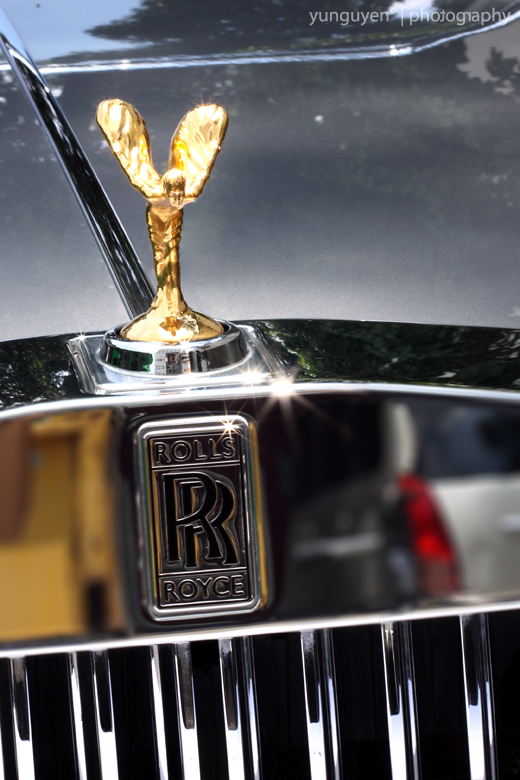
\includegraphics[height=0.85\paperheight]{images/yunguyen666_-_Rolls_Royce_-_cc-by-2_0_-_flickr}
		% Image source: https://www.flickr.com/photos/12716052@N04/3896880606/
		% Attribution watermark already included in image
		\hfil\hskip 2mm}\vfil}
\end{backgroundblock}
\begin{itemize}
\item Mercury administrator
\item Step creator
\item Pipeline creator
\item Pipeline runner
\end{itemize}
\end{frame}

%%%%%%%%%%%%%%%%%%%%%%%%%%%%%%%%%%%%%%%%
\subsection{System diagram}
\setbeamercolor*{background canvas}{bg=white}
\setbeamercolor{normal text}{fg=black, bg=white} 
\setbeamercolor*{example text}{fg=black} 
\setbeamercolor*{structure}{fg=sangerdarkblue} 
\begin{frame}{System \\
diagram}
\begin{backgroundblock}{0cm}{0cm}
		\vbox to \paperheight{\vfil\hbox to \paperwidth{\hskip 3cm 
		% Mercury system diagram is covered under the license for this work
		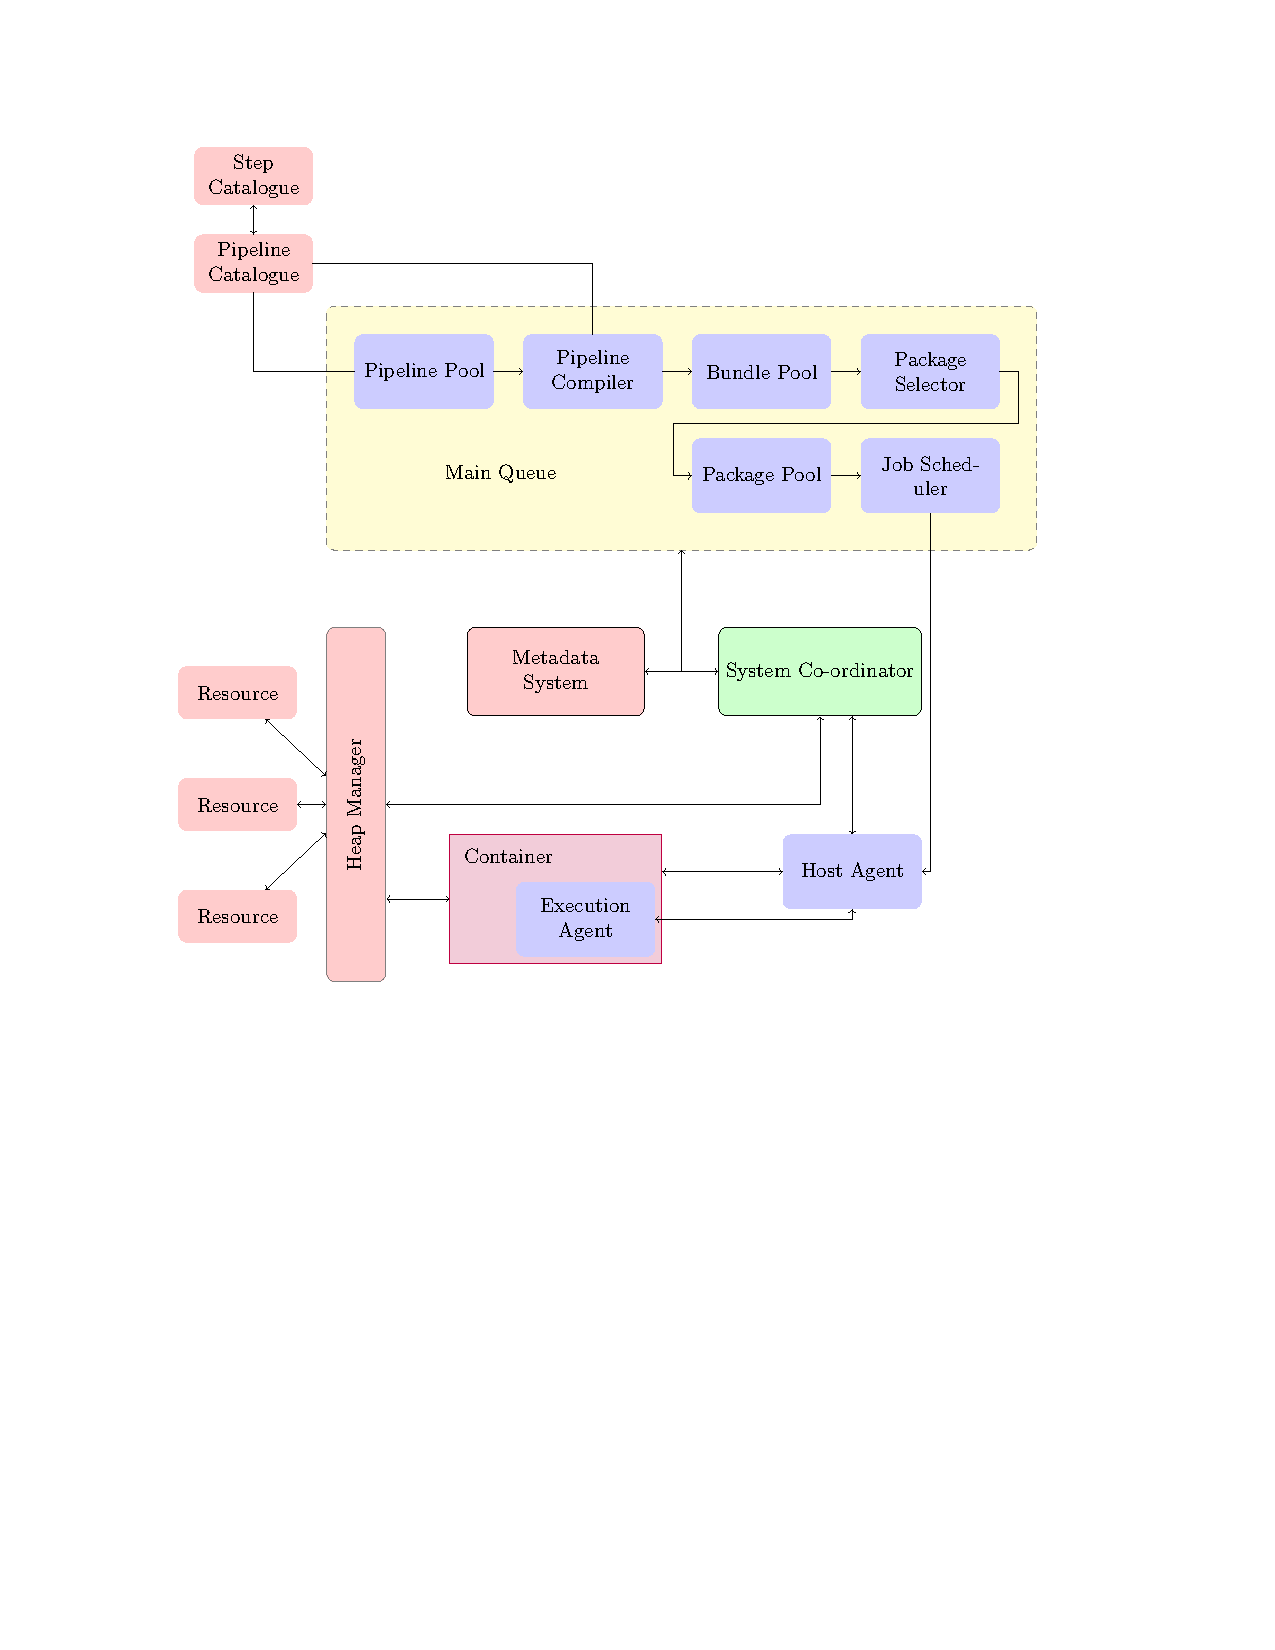
\includegraphics[height=0.85\paperheight]{images/mercury-system-diagram}
		\hfil\hskip 2mm}\vfil}
\end{backgroundblock}
\end{frame}


%%%%%%%%%%%%%%%%%%%%%%%%%%%%%%%%%%%%%%%%
% Questions
%%%%%%%%%%%%%%%%%%%%%%%%%%%%%%%%%%%%%%%%
\section*{\scshape Questions}
\setbeamercolor*{background canvas}{bg=black}
\setbeamercolor{normal text}{fg=white, bg=black} 
\setbeamercolor*{structure}{fg=sangermidblue} 
\begin{frame}{Questions?}
\end{frame}


\end{document}